% Intended LaTeX compiler: xelatex
\documentclass[a4paper, 12pt]{article}
\usepackage{graphicx}
\usepackage{longtable}
\usepackage{wrapfig}
\usepackage{rotating}
\usepackage[normalem]{ulem}
\usepackage{amsmath}
\usepackage{amssymb}
\usepackage{capt-of}
\usepackage{hyperref}
\usepackage[danish]{babel}
\usepackage{mathtools}
\usepackage[margin=3.0cm]{geometry}
\hypersetup{colorlinks, linkcolor=black, urlcolor=blue}
\setlength{\parindent}{0em}
\parskip 1.5ex
\author{Jacob Debel}
\date{Fysik C \& B}
\title{Lys og bølger\\\medskip
\large Refleksion - Eksperimenter}
\hypersetup{
 pdfauthor={Jacob Debel},
 pdftitle={Lys og bølger},
 pdfkeywords={},
 pdfsubject={},
 pdfcreator={Emacs 29.4 (Org mode 9.6.15)}, 
 pdflang={Danish}}
\begin{document}

\maketitle
Nu er I nået til refleksionsfasen, som er den sidste del i forløbet. I skulle gerne være eksperter inden for lysets brydning og det optiske gitter, både hvad angår kendskab og anvendelse af de tilhørende fagudtryk og matematiske udledninger af brydningsloven og gitterligningen. Jeres nye viden skal i bruge til at udføre eksperimenter.

\section*{Udførelse af eksperimenter}
\label{sec:org8605a7a}

\begin{itemize}
\item I får ca. 1.5 time i laboratoriet til at udføre jeres eksperimenter.

\item Husk at notere alle relevante målinger.

\item Husk at tage billeder af jeres forsøgsstillinger, som kan bruges I jeres rapport.
\end{itemize}

\newpage

\section*{Afrapportering}
\label{sec:org761334a}

I skal udarbejde en fysikrapport over jeres udførte eksperimenter. Afleveringsmappen ligger allerede på skolens it-platform. Husk følgende afsnit i rapporten:

\begin{itemize}
\item \textbf{Forord (I kan også kalde det formål)}

I skal skrive, hvad formålet med eksperimenterne er, og I skal opskrive hypoteser, hvis I har sådanne.

\item \textbf{Teori}

Her skal I have udledninger og forklaringer af gitterligningen og brydningsloven med.

\item \textbf{Forsøgsbeskrivelse}

Her skal I omskrive jeres fremgangsmåde til en forsøgsbeskrivelse. I skal skrive, hvad I faktisk har gjort i laboratoriet. Skriv det på punktform, men med hele sætninger. Indsæt også billeder af jeres opstillinger, eller hvis I ser noget, som er vigtigt for eksperimenterne.

\item \textbf{Resultater}

Her noteres eksperimentets "rå" data. Det kan være målte værdier sat op i en tabel, eller en graf over de samme værdier, hvis der er mange datapunkter. Det kan også være tale om billeder taget under eksperimentets udførelse, som senere skal bearbejdes.

\item \textbf{Databehandling}

Det er i dette afsnit, at alle beregninger på baggrund af data fra resultatafsnittet udføres.

\item \textbf{Diskussion}

Her sammenholdes de opnåede resultater af beregningerne med hypotesen fra formålsafsnittet. Det er også her, at der er plads til at fortolke på eksperimenterne og komme ind på eventuelle fejlkilder og usikkerheder. (Hvis der er tale om simple fejlkilder, så skal de ikke stå her. Så skal I udføre eksperimentet igen.)

\item \textbf{Konklusion}

Her skal hypotesen, resultater af beregninger samt diskussionen skrives sammen. Hvis man i hypotesen vil bestemme en talværdi for en bestemt fysisk størrelse, så skal tallet også være med her i konklusionen sammen med en relativ afvigelse.
\end{itemize}
\section*{Valg af eksperimenter}
\label{sec:org4a16140}

I skal udføre mindst 2 eksperimenter omkring lys og bølger. Eksperimenterne skal tilsammen omhandle brugen af \textbf{gitterligningen} og \textbf{brydningsloven}.

I de følgende afsnit er nogle korte introduktioner til mulige eksperimenter. I må meget gerne selv finde på andre eksperimenter.

Husk at udarbejde jeres egne forsøgsbeskrivelser, efter endt forsøg. Beskriv, hvad I faktisk har gjort.

\newpage
\subsection*{Bestemmelse af bølgelængde af laser}
\label{sec:org4514271}

\subsubsection*{Udstyr}
\label{sec:org9559c7d}
\begin{itemize}
\item Én laserpen (rød, grøn eller violet)
\item Ét optisk gitter (300, 600 eller 1200 linjer pr mm)
\item Lineal/målebånd/tommestok
\end{itemize}
\subsubsection*{Fremgangsmåde}
\label{sec:orgdb62576}
\begin{itemize}
\item Opstil eksperimentet så det ligner nogenlunde det følgende:
\end{itemize}

\begin{center}
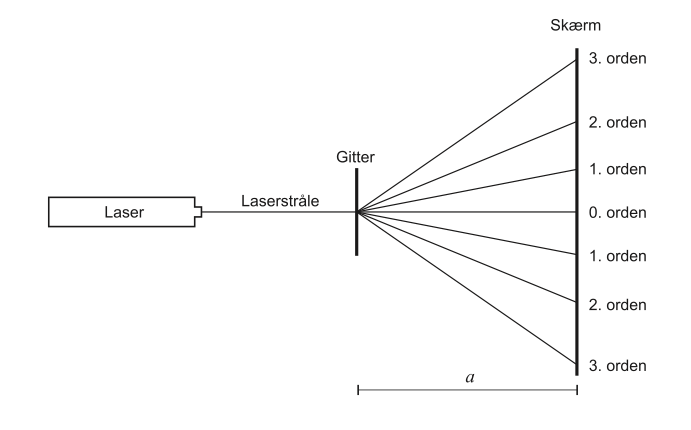
\includegraphics[width=.9\linewidth]{./img/boelgelaengde_laser.png}
\end{center}

\begin{itemize}
\item Mål afstanden mellem gitter og væg/skærm.
\item Mål afstanden mellem 0. orden og 1.orden. (Lav gerne et gennemsnit på begge sider af 0.orden.)
\end{itemize}

\subsubsection*{Databehandling}
\label{sec:org0622c0d}
\begin{itemize}
\item Beregn \(\phi_1\) fra \(\tan \left( \phi_1 \right) = \frac{x}{a}\).
\item Beregn \(\lambda\) fra \(\sin \left( \phi_{n} \right) = \frac{n \cdot \lambda}{d}\)
\end{itemize}

\newpage
\subsection*{Bestemmelse af gitterkonstant for CD eller DVD}
\label{sec:orga55ebc5}
\subsubsection*{Udstyr}
\label{sec:org0927eaf}
\begin{itemize}
\item Én laserpen (rød, grøn eller violet)
\item En CD eller DVD
\item Lineal/målebånd/tommestok
\end{itemize}
\subsubsection*{Fremgangsmåde}
\label{sec:orgd4e1459}
\begin{itemize}
\item Opstil eksperimentet så det ligner nogenlunde det følgende:
\end{itemize}

\begin{center}
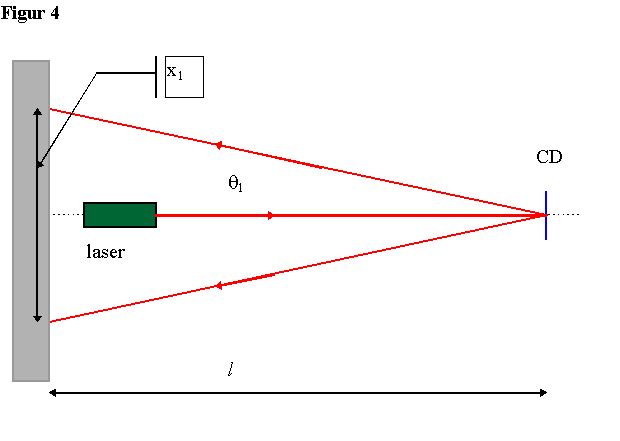
\includegraphics[width=.9\linewidth]{./img/gitterkonstant_cd_dvd.png}
\end{center}

\begin{itemize}
\item Mål afstanden mellem CD/DVD og væg/skærm.
\item Mål afstanden mellem 0. orden og 1.orden. (Lav gerne et gennemsnit på begge sider af 0.orden.)
\end{itemize}

\subsubsection*{Databehandling}
\label{sec:orgcdd7465}
\begin{itemize}
\item Beregn \(\theta_1\) fra \(\tan \left( \theta_1 \right) = \frac{x_1}{l}\).
\item Beregn \(d\) fra \(\sin \left( \theta_{n} \right) = \frac{n \cdot \lambda}{d}\)
\item Sammenlign gitterkonstanten for CD'en/DVD'en med de optiske gitre i laboratoriet.
\end{itemize}

\newpage
\subsection*{Bestemmelse af brydningsindeks for en væske}
\label{sec:org8a49f6c}
\subsubsection*{Udstyr}
\label{sec:org377a930}
\begin{itemize}
\item Én laserpen (rød, grøn eller violet)
\item Et gennemsigtigt kar.
\item Mobilkamera
\end{itemize}
\subsubsection*{Fremgangsmåde}
\label{sec:orgecfabf0}
\begin{itemize}
\item Opstil eksperimentet så det ligner nogenlunde det følgende:
\end{itemize}

\begin{center}
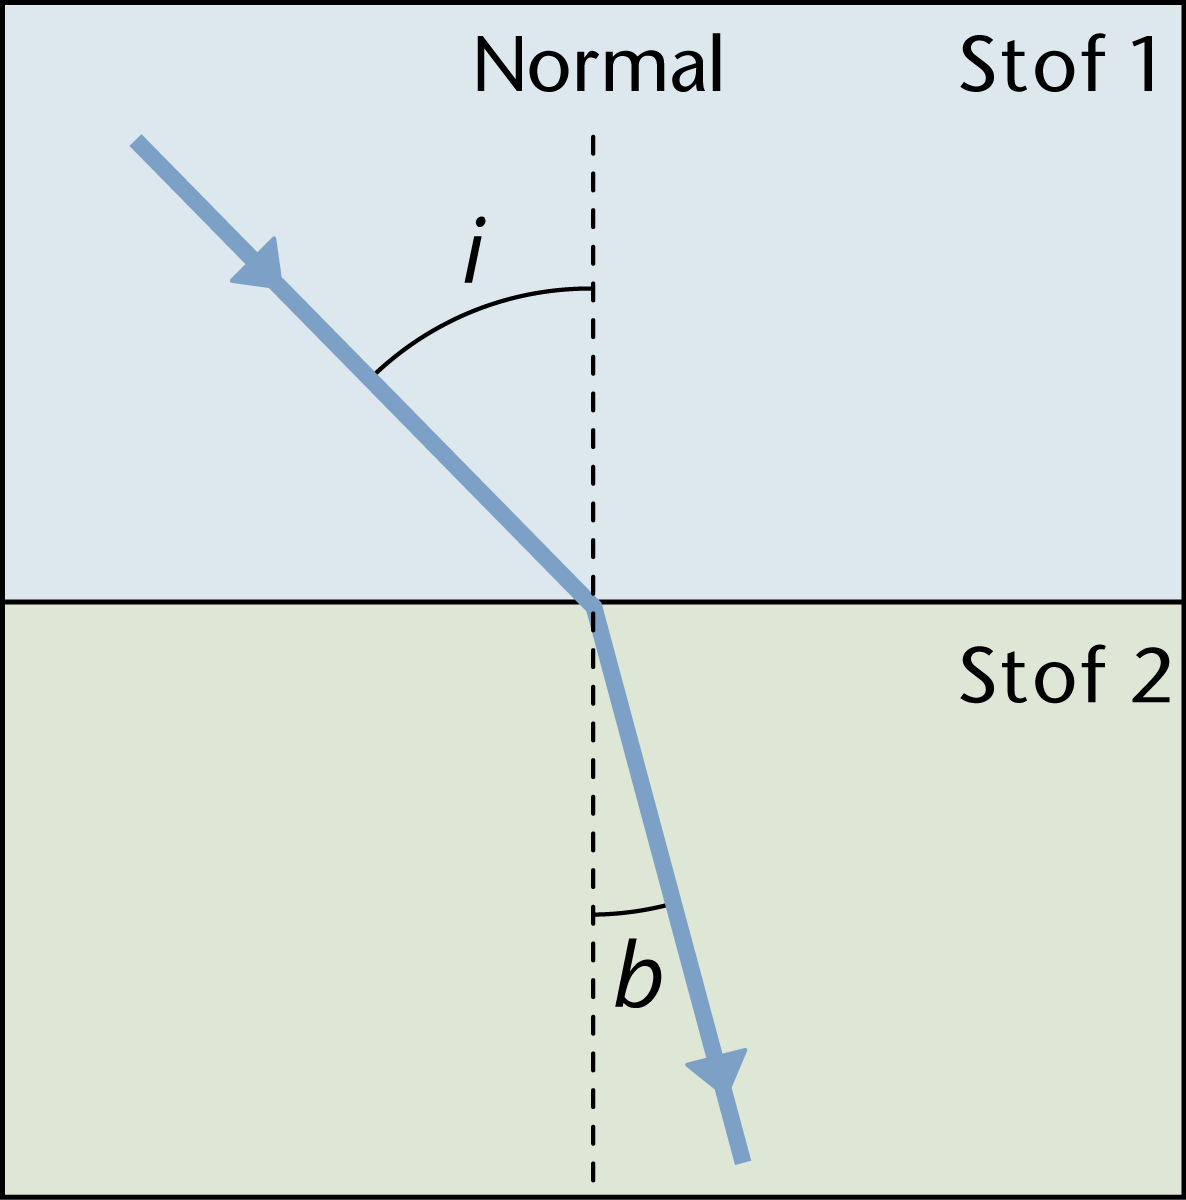
\includegraphics[width=0.5\linewidth]{./img/brydningsindeks_vaeske.png}
\end{center}

\begin{itemize}
\item Tag et billede af laserlysets strålegang med mobilkameraet. Det skal være så vinkelret på udbredelsen som muligt.
\end{itemize}

\subsubsection*{Databehandling}
\label{sec:orgd596a28}
\begin{itemize}
\item Overfør billedet til en computer.
\item Indsæt billedet i geogebra.
\item Opret en linje for væskeoverfladen.
\item Opret en vinkelret linje ift. væskeoverfladen.
\item Mål indfaldsvinkel og brydningsvinkel vha. geogebra.
\item Beregn \(n\) ud fra \(\frac{\sin(i)}{\sin(b)}=\frac{n_2}{n_1}\).
\end{itemize}

\newpage
\subsection*{Bestemmelse af brydningsindeks for glas eller akryl}
\label{sec:orgb0c7d45}

\subsubsection*{Udstyr}
\label{sec:orgd520018}
\begin{itemize}
\item Én laserpen (rød, grøn eller violet)
\item Et prisme/en klods af en eller anden form for glas eller akryl(plexiglas)
\item Mobilkamera
\end{itemize}
\subsubsection*{Fremgangsmåde}
\label{sec:org7c43fa2}
\begin{itemize}
\item Opstil eksperimentet så det ligner nogenlunde det følgende:
\end{itemize}

\begin{center}
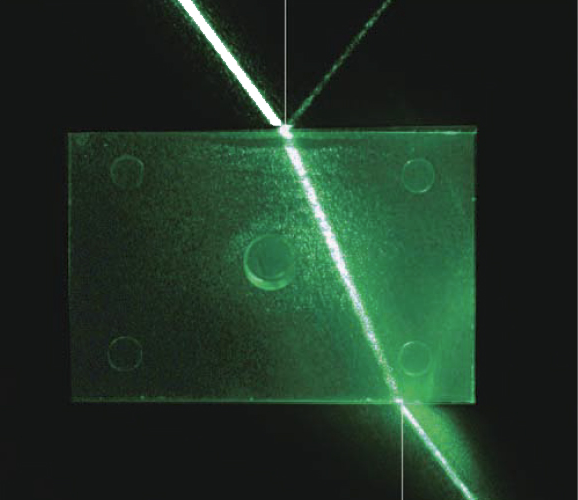
\includegraphics[width=0.5\linewidth]{./img/brydningsindeks_glas_akryl.png}
\end{center}

\begin{itemize}
\item Tag et billede af laserlysets strålegang med mobilkameraet. Det skal være så vinkelret på udbredelsen som muligt.
\end{itemize}

\subsubsection*{Databehandling}
\label{sec:org5ca686a}
\begin{itemize}
\item Overfør billedet til en computer.
\item Indsæt billedet i geogebra.
\item Opret en linje for grænsefladen mellem luft og klods.
\item Opret en vinkelret linje ift. grænsefladen.
\item Mål indfaldsvinkel og brydningsvinkel vha. geogebra.
\item Beregn \(n\) ud fra \(\frac{\sin(i)}{\sin(b)}=\frac{n_2}{n_1}\).
\end{itemize}

\newpage
\end{document}
